\section{Problem 5}

\subsection{Question}
Re-run question 2, but this time with proper TFIDF calculations instead of the hack discussed on slide 7 (p. 32).  Use the same 500 words, but this time replace their frequency count with TFIDF scores as computed in assignment \#3. Document the code, techniques, methods, etc. used to generate these TFIDF values.  Upload the new data file to github.\\
\\
Compare and contrast the resulting dendrogram with the dendrogram from question \#2.\\
\\
Note: ideally you would not reuse the same 500 terms and instead come up with TFIDF scores for all the terms and then choose the top 500 from that list, but I'm trying to limit the amount of work necessary.

\subsection{Answer}

To answer this question, {\tt matrix.py} was modified to add the capability to calculate {\it Term Frequency Inverse Document Frequency (TF/IDF)}. The added functions for computing TF/IDF are found in Listing \ref{listing:tfidf}. These functions use the master word count dictionary ({\tt wordcounts}) and each blog's individual word count ({\tt wc}) for each of the words in the {\tt wordlist} from Question 1/2 to compute the TF/IDF value for each word in the word list. 

\lstinputlisting[language=Python, caption={use of tfidf function},label=listing:tfidfmain,linerange={116-117},firstnumber=116]{matrix.py}

\lstinputlisting[language=Python, caption={writing the data}, label=listing:matrix:writedata, linerange={79-93}, firstnumber=79]{matrix.py}

\lstinputlisting[language=Python, caption={tf idf functions},label=listing:tfidf,linerange={40-48},
firstnumber=40]{matrix.py}

The same clustering was applied to the TF/IDF result matrix as was done in Question 2 and both images are displayed in Figures \ref{fig:raw} and \ref{fig:tfidf}.\\

There are a many pairs that were found to be similar in both clusterings. For example, in both dendrograms, the {\it Web Science and Digitial Libraries Research Group} blog is most similar to the {\it ...: zero pride and even less shame} blog, the {\it DJ DHANIEL FAN AND PRODUCER} is paired with {\it The Baron Boombox}, among a few others. In spite of this, the larger groupings do not appear very similar between the two clustings. There are some groups that share blogs in both dendrograms, but this is mostly due to there being only a few distinct groups in the raw count version and many of the TF/IDF clusters seemingly being subsets of the fewer, larger clustering from the raw count dendrogram.\\

When examining each of the clusters on a larger scale, it seems that the TF/IDF dendrogram clustered blogs are subjectively more alike than the raw count clusters. Looking toward the bottom of the TF/IDF clustering image, one will notice a grouping of blogs that seem closely related to music: {\it F-Measure: Less Than timely Music Reviews and Commentary.}, {\it Urban Anatomy's Columbian Jungle (That Dope!)} which seems to be a melding of fashion and music commentary, {\it Ezhevika Fields} a blog where info and preview samples of ``lost album samples of the past'' can be found, whereas these blogs are not all grouped together in the raw count dendrogram.\\

There is another cluster in the TF/IDF driven image that seems to contain family related blogs, with blogs like {\it Am I a funny girl?: I think I have my moments} which is, {\it The Frixen Family}, {\it When Two Hearts Become One: A wife, a mom, a daughter, a sibling.} and {\it The Clarks in Austin} all being related to a particular family and their everyday lives. Some of these blogs are close to each other in the raw count version, but they are not separated into their own distinct groups. The groups in the raw count version share some of these blogs, but are also mixed with others that seem unrelated. For example, the top cluster in the raw count dendrogram doesn't seem to have much of a unifying subject at all.\\

When looking at the overall structure of the two dendrograms it becomes apparent that there are more individual clusters grouped together in the TF/IDF version than are present in the raw count image, where there seems to be few small clusters and one mega-cluster in the center. This suggests that the TF/IDF algorithm was better at defining discrete subgroups within the larger context than the simple raw count dendrogram produced.

\begin{figure}[h!]
\centering
\fbox{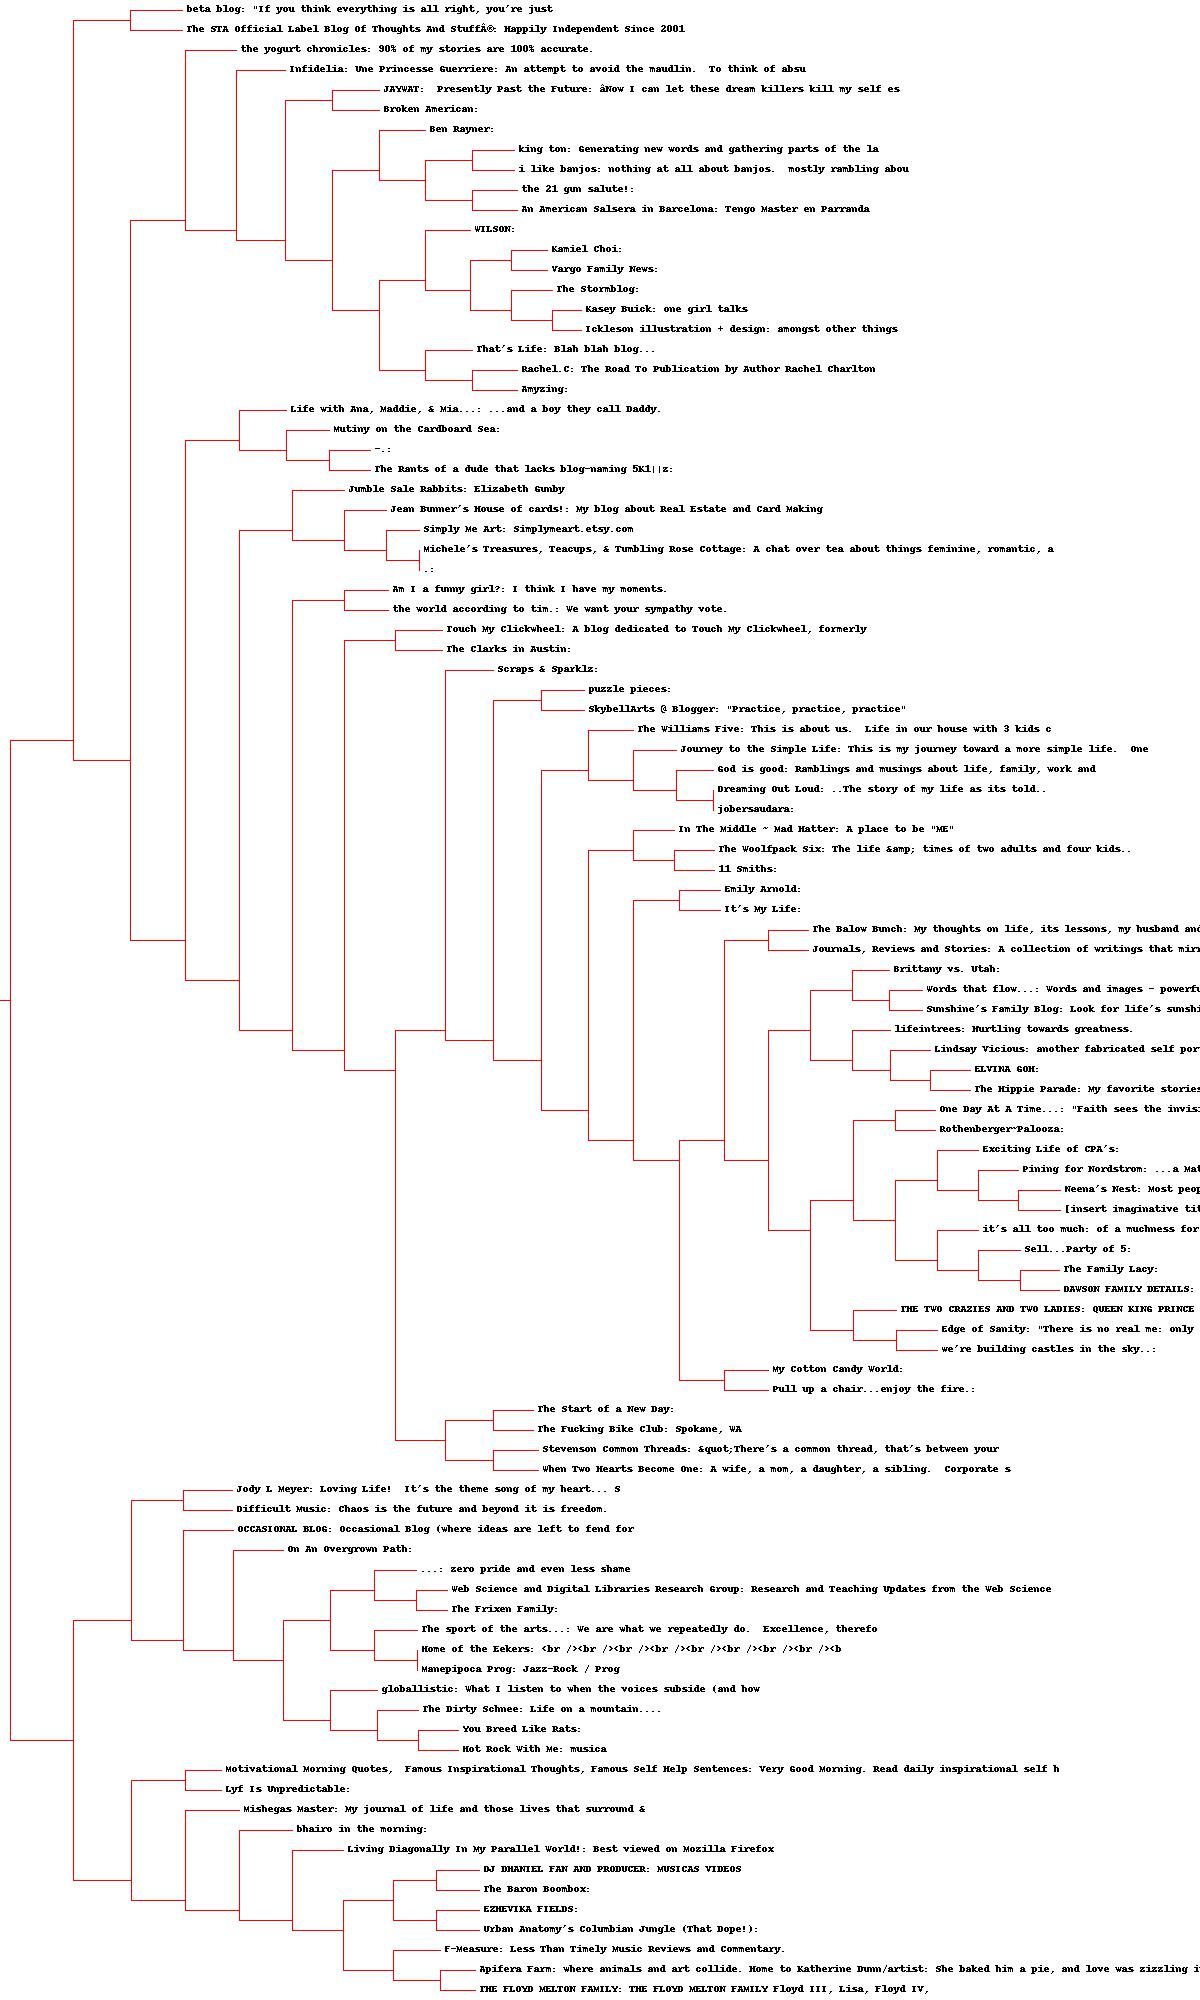
\includegraphics[scale=0.3]{q2/blogclust.jpg}}
\caption{raw count dendrogram}
\label{fig:raw}
\end{figure}

\begin{figure}[h!]
\centering
\fbox{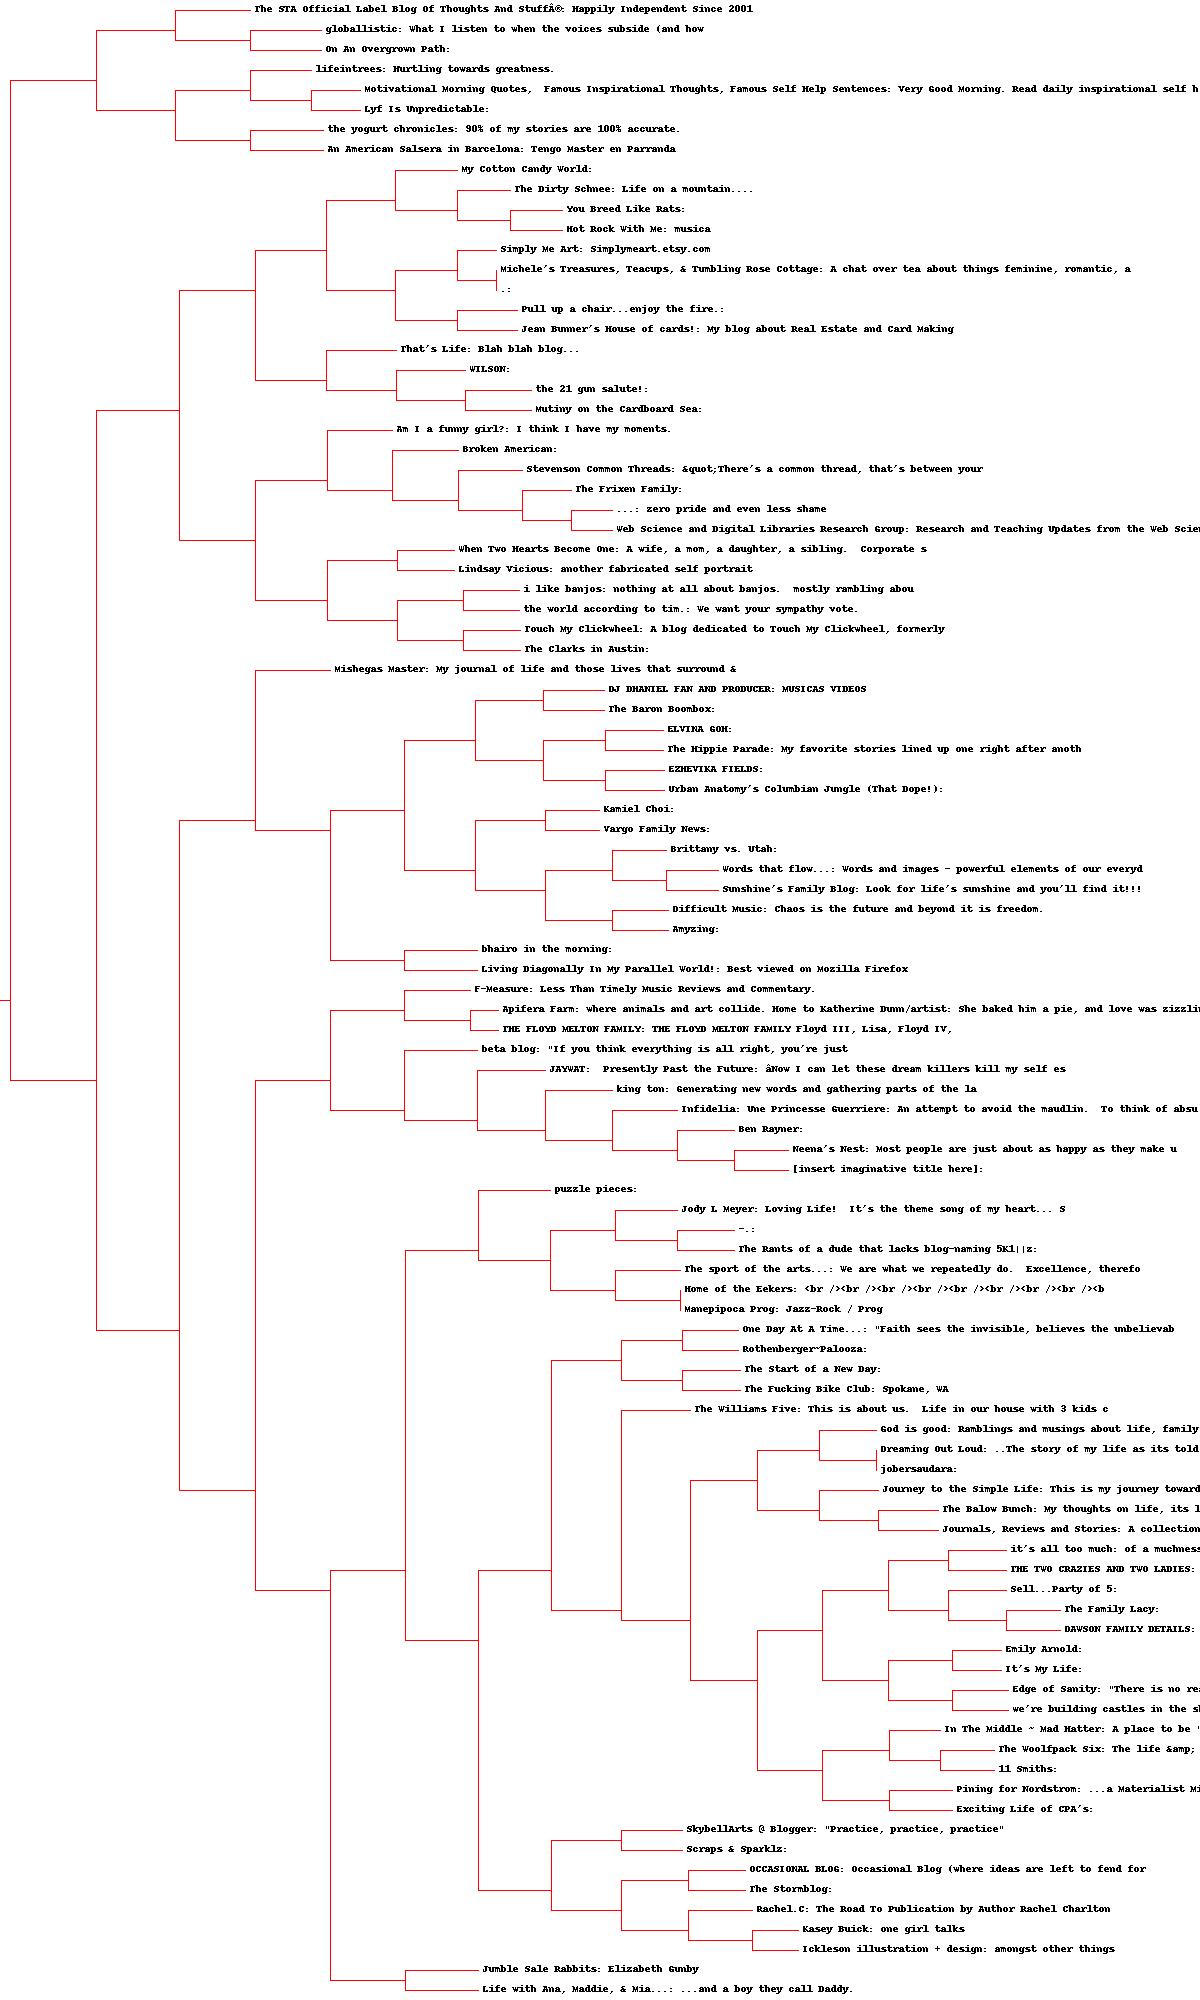
\includegraphics[scale=0.3]{q5/blogclust.jpg}}
\caption{TF/IDF dendrogram}
\label{fig:tfidf}
\end{figure}